% Romer (2012), Problem 4.8, p. 186 -- solution fragment for hardest-solutions.tex (statement not reproduced).
% Every key result is re-checked by hardest-parts/check-4-8-8-1.py.
\problema{Romer 4.8}{Physical and human capital with an education sector}{p.~186}{Romer \S4.1}

\noindent\textit{Notation.} $x_K\equiv n+g+\delta_K$, $x_H\equiv n+g+\delta_H$,
$c_K\equiv s(1-a_K)^{\alpha}(1-a_H)^{1-\alpha}$ and $c_H\equiv B\,a_K^{\gamma}a_H^{\phi}$. $L$ counts people (bodies), so
``per person'' means per unit of $L$. Throughout, $0<\alpha<1$, $0<a_K,a_H<1$, $\gamma,\phi>0$ and $\gamma+\phi<1$.

\parte{a}
\passo{growth-rate identity}{Take logs of $k=K/(AL)$, $\ln k=\ln K-\ln A-\ln L$, and differentiate with respect to
time, using $\dot A/A=g$ and $\dot L/L=n$:
\[ \frac{\dot k}{k}=\frac{\dot K}{K}-g-n\quad\Longrightarrow\quad\dot k=\frac{\dot K}{AL}-(n+g)\,k;
\qquad\text{likewise}\qquad\dot h=\frac{\dot H}{AL}-(n+g)\,h. \]}
\passo{goods per unit of effective labor}{The exponents of the goods technology sum to one, so dividing by
$AL=(AL)^{\alpha}(AL)^{1-\alpha}$,
\[ y\equiv\frac{Y}{AL}=\Big[(1-a_K)\frac{K}{AL}\Big]^{\alpha}\Big[(1-a_H)\frac{H}{AL}\Big]^{1-\alpha}
=(1-a_K)^{\alpha}(1-a_H)^{1-\alpha}\,k^{\alpha}h^{1-\alpha}. \]}
\passo{law of motion of $k$}{$\dot K/(AL)=sY/(AL)-\delta_KK/(AL)=sy-\delta_Kk$; substituting into the identity,
\[ \dot k=c_K\,k^{\alpha}h^{1-\alpha}-x_K\,k. \]}
\passo{law of motion of $h$}{The education technology is homogeneous of degree one in $(K,H,AL)$; dividing it by
$AL=(AL)^{\gamma}(AL)^{\phi}(AL)^{1-\gamma-\phi}$,
\[ \begin{aligned}
\frac{\dot H}{AL}+\delta_Hh&=B\,a_K^{\gamma}a_H^{\phi}\Big(\frac{K}{AL}\Big)^{\gamma}\Big(\frac{H}{AL}\Big)^{\phi}
\Big(\frac{AL}{AL}\Big)^{1-\gamma-\phi}=c_H\,k^{\gamma}h^{\phi},\\
\dot h&=c_H\,k^{\gamma}h^{\phi}-x_H\,h.
\end{aligned} \]}

\parte{b}
\passo{the $\dot k=0$ locus}{For $k>0$, $\dot k=0$ iff $c_Kk^{\alpha-1}h^{1-\alpha}=x_K$, i.e.\ $(h/k)^{1-\alpha}=x_K/c_K$.
Raising both sides to the power $-1/(1-\alpha)$:
\[ \dot k=0\iff k=\kappa\,h,\qquad\kappa\equiv\Big(\frac{c_K}{x_K}\Big)^{1/(1-\alpha)}. \]
In $(h,k)$ space ($h$ on the horizontal axis) this is a ray through the origin with slope $\kappa>0$: goods
production has constant returns in $K$ and $H$, so only the ratio $h/k$ matters for $\dot k/k$. Off the locus,
$\dot k=k\,[c_K(h/k)^{1-\alpha}-x_K]$, and for given $h$ the bracket falls with $k$: $\dot k<0$ above the ray, $\dot k>0$
below it.}
\passo{the $\dot h=0$ locus}{For $h>0$, $\dot h=0$ iff $c_Hk^{\gamma}=x_Hh^{1-\phi}$; raising to the power $1/\gamma$,
\[ \dot h=0\iff k=\lambda\,h^{\eta},\qquad\lambda\equiv\Big(\frac{x_H}{c_H}\Big)^{1/\gamma},\qquad
\eta\equiv\frac{1-\phi}{\gamma}>1, \]
where $\eta>1$ is exactly the assumption $\gamma+\phi<1$. Differentiating,
\[ \frac{dk}{dh}=\eta\lambda h^{\eta-1}>0,\qquad\frac{d^2k}{dh^2}=\eta(\eta-1)\lambda h^{\eta-2}>0, \]
so the locus leaves the origin with zero slope ($\eta-1>0$), is increasing and strictly convex, and its slope tends
to infinity as $h\to\infty$; equivalently, $h=(c_Hk^{\gamma}/x_H)^{1/(1-\phi)}$ is a concave function of $k$, since
$\gamma/(1-\phi)<1$. Off the locus, $\dot h=h\,[c_Hk^{\gamma}h^{\phi-1}-x_H]$ rises with $k$: $\dot h>0$ above the
curve, $\dot h<0$ below it.}

\begin{center}
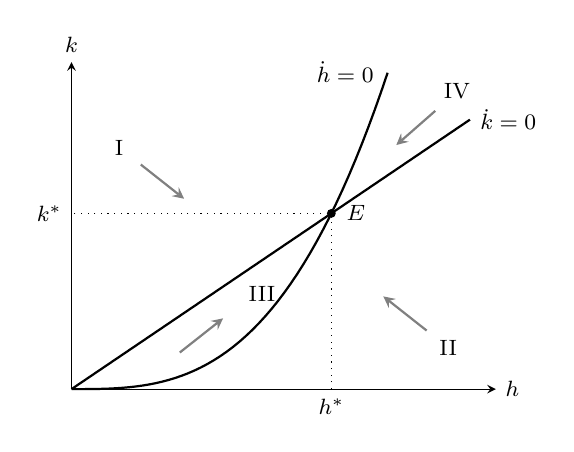
\begin{tikzpicture}[x=1.1cm,y=0.62cm,font=\footnotesize,>=stealth]
  \draw[->] (0,0) -- (4.9,0) node[right] {$h$};
  \draw[->] (0,0) -- (0,6.7) node[above] {$k$};
  \draw[thick] (0,0) -- (4.6,5.52) node[right] {$\dot k=0$};
  \draw[thick,domain=0:3.65,samples=50] plot (\x,{2/15*\x*\x*\x});
  \node[left] at (3.6,6.5) {$\dot h=0$};
  \draw[dotted] (3,0) node[below] {$h^*$} -- (3,3.6) -- (0,3.6) node[left] {$k^*$};
  \fill (3,3.6) circle (1.6pt) node[right=2pt] {$E$};
  \draw[->,thick,gray] (0.8,4.6) -- (1.3,3.9);    \node at (0.55,4.95) {I};
  \draw[->,thick,gray] (4.1,1.2) -- (3.6,1.9);    \node at (4.35,0.85) {II};
  \draw[->,thick,gray] (1.25,0.75) -- (1.75,1.45); \node at (2.2,1.95) {III};
  \draw[->,thick,gray] (4.2,5.7) -- (3.75,5.0);   \node at (4.45,6.1) {IV};
\end{tikzpicture}\\[2pt]
{\footnotesize Figure 4.8-1. The $\dot k=0$ ray, the convex $\dot h=0$ locus, and the direction of motion in
each region.}
\end{center}

\parte{c}
\passo{existence and uniqueness}{A balanced growth path is a rest point with $k,h>0$, i.e.\ a point on both loci:
$\kappa h=\lambda h^{\eta}\iff h^{\eta-1}=\kappa/\lambda$. As $\eta-1=(1-\gamma-\phi)/\gamma>0$, $h^{\eta-1}$ rises
strictly from $0$ to $\infty$, so there is exactly one positive solution,
\[ \begin{aligned}
h^*&=\Big(\frac{\kappa}{\lambda}\Big)^{\frac{\gamma}{1-\gamma-\phi}}
=\Big(\frac{c_K}{x_K}\Big)^{\frac{\gamma}{(1-\alpha)(1-\gamma-\phi)}}\Big(\frac{c_H}{x_H}\Big)^{\frac{1}{1-\gamma-\phi}},\\
k^*&=\kappa h^*=\Big(\frac{c_K}{x_K}\Big)^{\frac{1-\phi}{(1-\alpha)(1-\gamma-\phi)}}\Big(\frac{c_H}{x_H}\Big)^{\frac{1}{1-\gamma-\phi}},
\end{aligned} \]
where the exponent of $c_K/x_K$ in $k^*$ is $\frac{1}{1-\alpha}+\frac{\gamma}{(1-\alpha)(1-\gamma-\phi)}
=\frac{1-\phi}{(1-\alpha)(1-\gamma-\phi)}$. Since $\eta>1$, the ray lies above the curve for $0<h<h^*$ and below it
for $h>h^*$. The origin is the only other rest point, and the next step shows it attracts no path with $k_0,h_0>0$.}
\passo{global stability: phase diagram}{The loci cut the positive quadrant into four regions (Figure 4.8-1):
I above both ($\dot h>0$, $\dot k<0$), II below both ($\dot h<0$, $\dot k>0$), III between them with $h<h^*$
($\dot h>0$, $\dot k>0$), IV between them with $h>h^*$ ($\dot h<0$, $\dot k<0$). On the ray bounding III, $\dot k=0$
and $\dot h>0$, so the flow points right, into III; on the curve bounding III, $\dot h=0$ and $\dot k>0$, so it points
up, into III. Hence a path never leaves III, and likewise IV. In III, $k$ and $h$ rise and stay below $k^*,h^*$; in IV
they fall and stay above them; a monotone bounded path converges, and its limit must be a rest point: $E$. In I, $h$
rises and $k$ falls with $\lambda h_0^{\eta}\le\lambda h^{\eta}<k\le k_0$ and $h<k/\kappa\le k_0/\kappa$: the path either
enters III or IV or stays in I bounded away from $0$ and $\infty$, and converges to $E$ in both cases. II is symmetric
($k_0\le k<\kappa h\le\kappa h_0$ and $h>(k_0/\lambda)^{1/\eta}$). So every path with $k_0,h_0>0$ converges to $E$:
the balanced growth path exists, is unique, and is globally stable.}
\passo{local stability: Jacobian}{Using the locus conditions $c_Kk^{\alpha-1}h^{1-\alpha}=x_K$ and
$c_Hk^{\gamma}h^{\phi-1}=x_H$ at $E$,
\[ \begin{aligned}
\frac{\partial\dot k}{\partial k}&=\alpha c_Kk^{\alpha-1}h^{1-\alpha}-x_K=-(1-\alpha)x_K,&
\frac{\partial\dot k}{\partial h}&=(1-\alpha)c_Kk^{\alpha-1}h^{1-\alpha}\,\frac kh=(1-\alpha)x_K\frac{k^*}{h^*},\\
\frac{\partial\dot h}{\partial k}&=\gamma c_Hk^{\gamma}h^{\phi-1}\,\frac hk=\gamma x_H\frac{h^*}{k^*},&
\frac{\partial\dot h}{\partial h}&=\phi c_Hk^{\gamma}h^{\phi-1}-x_H=-(1-\phi)x_H.
\end{aligned} \]
Hence, since the ratios $k^*/h^*$ cancel in the determinant,
\[ \begin{aligned}
\operatorname{tr}J&=-(1-\alpha)x_K-(1-\phi)x_H<0,\\
\det J&=(1-\alpha)(1-\phi)x_Kx_H-(1-\alpha)\gamma\,x_Kx_H=(1-\alpha)(1-\gamma-\phi)\,x_Kx_H>0,\\
(\operatorname{tr}J)^2-4\det J&=\big[(1-\alpha)x_K+(1-\phi)x_H\big]^2-4(1-\alpha)(1-\phi)x_Kx_H+4(1-\alpha)\gamma\,x_Kx_H\\
&=\big[(1-\alpha)x_K-(1-\phi)x_H\big]^2+4(1-\alpha)\gamma\,x_Kx_H>0.
\end{aligned} \]
Two real negative eigenvalues: $E$ is a stable node (no oscillations), and the eigenvalue closer to zero sets the
asymptotic speed of convergence. Again $\det J>0$ is the assumption $\gamma+\phi<1$.}
\passo{growth rates on the balanced path}{With $k=k^*$ and $h=h^*$ constant, $K=k^*AL$, $H=h^*AL$ and $Y=y^*AL$ all
grow at $n+g$, and per person
\[ \frac KL=A\,k^*,\qquad\frac HL=A\,h^*,\qquad\frac YL=A\,y^*,\qquad
y^*=(1-a_K)^{\alpha}(1-a_H)^{1-\alpha}k^{*\alpha}h^{*1-\alpha}, \]
so output, physical capital and human capital per person all grow at rate $g$.}
\intuicao{$K$ helps produce $H$ and $H$ helps produce goods, hence $K$; but the feedback dies out because education
also uses $AL$, which cannot be accumulated, and $\gamma+\phi<1$ means diminishing returns to $K$ and $H$ together.
As in Solow, long-run growth per person is the exogenous $g$.}
\armadilha{The condition $\gamma+\phi<1$ does all the work. With $\gamma+\phi=1$, $\eta=1$ and the $\dot h=0$ locus is
also a ray; the two rays generically meet only at the origin, there is no rest point with $k,h>0$, and $K$ and $H$
grow at a rate that depends on $s$, $a_K$, $a_H$ and $B$: an endogenous-growth model (compare Problem 4.9).}

\parte{d}
\passo{which locus moves}{$s$ enters only $c_K$, hence only $\kappa=(c_K/x_K)^{1/(1-\alpha)}$: a permanent rise from
$s$ to $s'>s$ makes the $\dot k=0$ ray steeper and leaves the $\dot h=0$ curve unchanged. The new intersection $E'$
has higher $h^*$ and $k^*$, since both exponents of $c_K$ in part (c) are positive.}
\passo{the transition}{$k$ and $h$ are stocks, so at the date of the change, $t_0$, the economy is still at $E$, which
is on the unchanged $\dot h=0$ curve and now strictly below the new ray:
\[ \dot h(t_0)=0,\qquad\frac{\dot k(t_0)}{k^*}=\frac{s'}{s}\,c_Kk^{*\alpha-1}h^{*1-\alpha}-x_K=\Big(\frac{s'}{s}-1\Big)x_K>0. \]
The economy enters region III of the new diagram and never leaves it: $k$ and $h$ rise monotonically and converge to
$E'$, asymptotically rather than at a finite date. At first only $k$ moves (the path starts vertically); then $h$ rises
as more $K$ flows into schooling (Figure 4.8-2, left).}
\passo{output per person}{$\ln(Y/L)=\ln A+\ln y$, with $\ln y$ equal to a constant plus $\alpha\ln k+(1-\alpha)\ln h$, so
\[ \frac{d\ln(Y/L)}{dt}=g+\alpha\frac{\dot k}{k}+(1-\alpha)\frac{\dot h}{h}. \]
At $t_0$ the level does not jump ($k$ and $h$ are predetermined); its growth rate jumps from $g$ to
$g+\alpha(s'/s-1)x_K$, stays above $g$ throughout the transition ($\dot k,\dot h\ge0$, not both zero), and returns to
$g$ as $E'$ is approached. The decline need not be monotone. At $t_0$, where $\dot h=0$,
\[ \begin{aligned}
\frac{d}{dt}\frac{\dot k}{k}&=(1-\alpha)\frac{s'}{s}c_K\Big(\frac hk\Big)^{1-\alpha}\Big(\frac{\dot h}{h}-\frac{\dot k}{k}\Big)
=-(1-\alpha)\frac{s'}{s}x_K\,\frac{\dot k}{k},\\
\frac{d}{dt}\frac{\dot h}{h}&=c_Hk^{\gamma}h^{\phi-1}\Big(\gamma\frac{\dot k}{k}-(1-\phi)\frac{\dot h}{h}\Big)
=\gamma x_H\,\frac{\dot k}{k},\\
\frac{d}{dt}\Big[\alpha\frac{\dot k}{k}+(1-\alpha)\frac{\dot h}{h}\Big]_{t_0}
&=(1-\alpha)\Big(\frac{s'}{s}-1\Big)x_K\Big[\gamma x_H-\alpha\frac{s'}{s}x_K\Big],
\end{aligned} \]
so growth first accelerates when $\gamma x_H>\alpha(s'/s)x_K$: the education channel kicks in with a lag. In the
long run $\ln(Y/L)$ is higher, by the elasticity below times the change in $\ln s$, and grows at $g$ again:
\[ \frac{d\ln y^*}{d\ln s}=\alpha\frac{1-\phi}{(1-\alpha)(1-\gamma-\phi)}+(1-\alpha)\frac{\gamma}{(1-\alpha)(1-\gamma-\phi)}
=\frac{\alpha}{1-\alpha}+\frac{\gamma}{(1-\alpha)(1-\gamma-\phi)}. \]}

\begin{center}
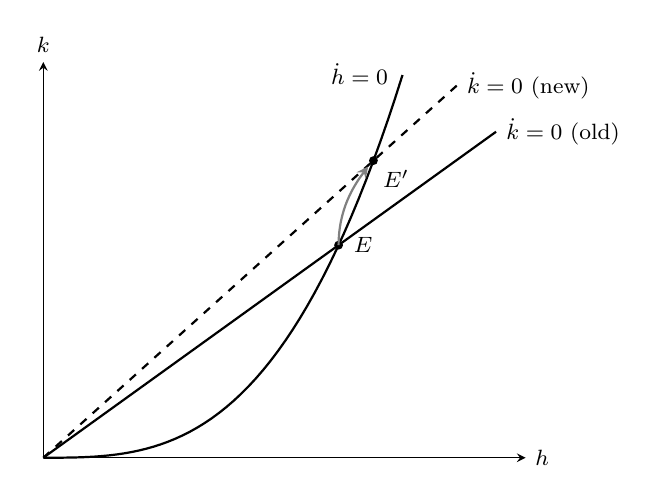
\begin{tikzpicture}[x=1.25cm,y=0.75cm,font=\footnotesize,>=stealth]
  \draw[->] (0,0) -- (4.9,0) node[right] {$h$};
  \draw[->] (0,0) -- (0,6.7) node[above] {$k$};
  \draw[thick] (0,0) -- (4.6,5.52) node[right] {$\dot k=0$ (old)};
  \draw[thick,dashed] (0,0) -- (4.2,6.3) node[right] {$\dot k=0$ (new)};
  \draw[thick,domain=0:3.65,samples=50] plot (\x,{2/15*\x*\x*\x});
  \node[left] at (3.6,6.5) {$\dot h=0$};
  \fill (3,3.6) circle (1.6pt) node[right=2pt] {$E$};
  \fill (3.354,5.031) circle (1.6pt) node[below right] {$E'$};
  \draw[->,thick,gray] (3,3.6) .. controls (3,4.2) and (3.15,4.6) .. (3.3,4.93);
\end{tikzpicture}\qquad
\begin{tikzpicture}[x=0.85cm,y=0.95cm,font=\footnotesize,>=stealth]
  \draw[->] (0,0) -- (6.8,0) node[right] {$t$};
  \draw[->] (0,0) -- (0,4.1) node[above] {$\ln(Y/L)$};
  \draw[thick] (0,0.8) -- (2,1.4);
  \draw[dashed] (2,1.4) -- (6.3,2.69);
  \draw[dotted] (2,2.3) -- (6.3,3.59);
  \draw[thick,domain=2:6.3,samples=50] plot (\x,{0.8+0.3*\x+0.9*(1-exp(-0.9*(\x-2)))});
  \draw (2,0.08) -- (2,-0.08) node[below] {$t_0$};
\end{tikzpicture}\\[2pt]
{\footnotesize Figure 4.8-2. Left: the rise in $s$ steepens the $\dot k=0$ ray; the economy moves from $E$ to $E'$
inside the new region III. Right: $\ln(Y/L)$ (solid) does not jump at $t_0$, grows faster than $g$ during the
transition, and approaches a path parallel to the old one (dashed) but higher (dotted).}
\end{center}

\intuicao{A higher $s$ raises $K$, which raises goods output directly, as in Solow, and also raises the inputs to
schooling and hence $H$: a second round of accumulation that Solow lacks. That is why the long-run elasticity
exceeds the Solow value $\alpha/(1-\alpha)$ by $\gamma/[(1-\alpha)(1-\gamma-\phi)]$. Neither round changes long-run
growth, which is pinned down by $g$: a level effect, not a growth effect.}
\armadilha{Two common slips: letting output per person jump at $t_0$ (only its growth rate jumps, because $k$ and
$h$ are stocks), and having the economy reach $E'$ at a finite date (convergence is asymptotic).}
\refbib{Romer (2012), \S4.1, pp.~151--156 (human capital in the Solow framework; the intensive-form method of
eq.~(4.7)); \S1.3--1.5, pp.~15--26 (Solow dynamics and the level effect of $s$); Problem 4.9 and Lucas (1988) for the
endogenous-growth case.}
\checado{\texttt{check-4-8-8-1.py} verifies the laws of motion from the levels, both loci and the signs off them,
$k^*$ and $h^*$, the Jacobian's trace, determinant and discriminant, growth at $g$ on the balanced path (simulated in
levels), the jump and initial slope of growth after a rise in $s$, the $s$-elasticity, monotone convergence to $E'$
and convergence from 20 random starting points. The solution manual agrees on (a)--(d); its sketch has the economy
reach $E'$ at a finite date $t_1$, whereas convergence is only asymptotic.}
